\section{\mbox{Data Source}}
\label{sec:data}
% Comcast dataset quick overview, dates, usage, tiers
Our dataset consists of network usage byte counters reported by Comcast gateways every 15 minutes from October 1, 2014 to December 29, 2014. There are two sets of broadband tiers that were used to collect this data: \control set, consisting of homes and businesses with a 105 Mbps access link, and the \test set, consisting of homes and businesses that were paying for a 105 Mbps access link, yet were receiving 250 Mbps instead. Users in the test set were selected randomly and were not told that their access bandwidth has been increased. There were more than 15000 gateway devices in the control set, with varying usage over the three months, and about 2200 gateway devices in the test set.
% test 2200 are unsanitized, after is 1481
% control ?? unsanitized. control4 itself has 15000 for the first 6 days that drops to 5k later. 16015 is after sanitization
\todo{confirm - these were reported by Comcast gateways right?}

% Representativeness of dataset
Both the \test and \control sets were collected from users in Salt Lake City, Utah, to avoid any biases in behavior based on location. Although this dataset corresponds to just one ISP, we believe that it is broadly representative of urban users in the US in the same, or higher broadband bandwidth tier ($\>$ 100 Mbps). Thus, we use this data to draw general conclusions about behavioral change with link capacity \todo{(add more here...) }

% use bismark passive data for passive patterns on different tiers - utilization like peeking paper
% active data for latency measurements to some central server during peak hours
\sg{Supplement the data with bismark?}

% mobile usage during peak vs non peak, user classification: wifi, 4g, tethering. Apps using most data
\sg{My Speed Test Usage Patterns data - Any chance?}

\subsection{Data Description}

%8 control sets, different devices, different times
%more details about data, fields, direction, locations?
Comcast splits the \control set into 8 separate pools on different date ranges and gateways \todo{confirm if there is repeated device IDs in control1-8.}. Each dataset contains the following relevant fields: Device ID, sample period time, service class, service direction, IP address, and the bytes transferred in the 15 minute sample slot, as described in table~\ref{tab:field-description}. \todo{find out more about service class name, and IP addresses being the same across all sets}

%\begin{table}[ht]
%\small
%\begin{tabular}{|l|l|}
%\hline
%\textbf{Field}         & \textbf{Description}                      \\ \hline
%Device\_number         & Arbitrarily assigned CM device identifier \\ \hline
%end\_time              & Fifteen minute sample period end time     \\ \hline
%date\_service\_created & Service start (not used in our analysis)  \\ \hline
%service\_class\_name   & Used to differentiate data application    \\ \hline
%cmts\_inet             & Cmts identifier (derived from ip address) \\ \hline
%service\_direction     & 1-downstream, 2-upstream                  \\ \hline
%port\_name             & Cmts port descriptor                      \\ \hline
%octets\_passed         & Byte count                                \\ \hline
%device\_key            & not used in our analysis                  \\ \hline
%service\_identifier    & Service id (not used in our analysis)     \\ \hline
%\end{tabular}
%\caption{Field Descriptions for Comcast Dataset by Comcast}
%\label{tab:field-description}
%\end{table}


\begin{table}[ht]
\small
\begin{tabular}{|l|l|}
\hline
\textbf{Field}         & \textbf{Description}                      \\ \hline
Device\_number         & Arbitrarily assigned CM device identifier \\ \hline
end\_time              & Fifteen minute sample period end time     \\ \hline
cmts\_inet             & Cmts identifier (derived from ip address) \\ \hline
service\_direction     & 1-downstream, 2-upstream                  \\ \hline
octets\_passed         & Byte count                                \\ \hline
\end{tabular}
\caption{Field Descriptions for Comcast Dataset by Comcast}
\label{tab:field-description}
\end{table}

\subsection{Data Processing}

% split database by direction, combine service class name
To process the large amount of data (more than 15000 unique devices, 96 time slots per day, 3 months, multiple service classes per time-slot), we first split the data by direction into uplink and downlink. The nature of the questions we ask in section~\ref{sec:intro} encourages us to concentrate on the downstream data, although we present similar results for upstream data in section~\ref{sec:results}. We also do not use the service class name identifier in our analysis, which is internal to Comcast. \todo{Our analysis showed that ignoring the service class identifier does not change our conclusions on usage patterns and statistics.} Thus we only considered overall usage for each gateway device in each time slot, in uplink and downlink direction.

%granularity of 15 mins, usually not perfectly synchronized but off by a very few seconds that shouldn't matter much when seeing larger aggregated patterns
Note that 15 minute time slots were synchronized to the same time stamp. They were off only by a few seconds (under 30, as claimed by Comcast). As our analysis deals with aggregated patterns on a granularity of 15 minutes, we believe this time synchronization to be irrelevant.

\subsection{Data Sanitization}

%\sg{correlated drops at times or devices that contributed only 2-3 days of the whole month}
Our initial analysis of data transferred per time slot showed that certain gateway devices were responsive only for brief periods. We also noticed that certain time slots had a very low response rate throughout the dataset. \todo{Why? asked comcast}.

%\sg{remove machines that contribute to less than 0.8 of the time slots.}
We evaluate the fraction of responsiveness of a gateway throughout the dataset, as well as the fraction of responsiveness per time slot, and call this the \textbf{availability}. Figure~\ref{fig:availability} shows how the number of devices decreases for a higher availability requirement. Based on the common trend of this plot throughout the \test and \control datasets, we decided to only choose gateway devices with an availability of at least 0.8.


\begin{figure}[t!]
%\hspace*{-0.2in}
\begin{minipage}{1\linewidth}
\centering
%
%\hfill
\begin{subfigure}[b]{0.5\linewidth}
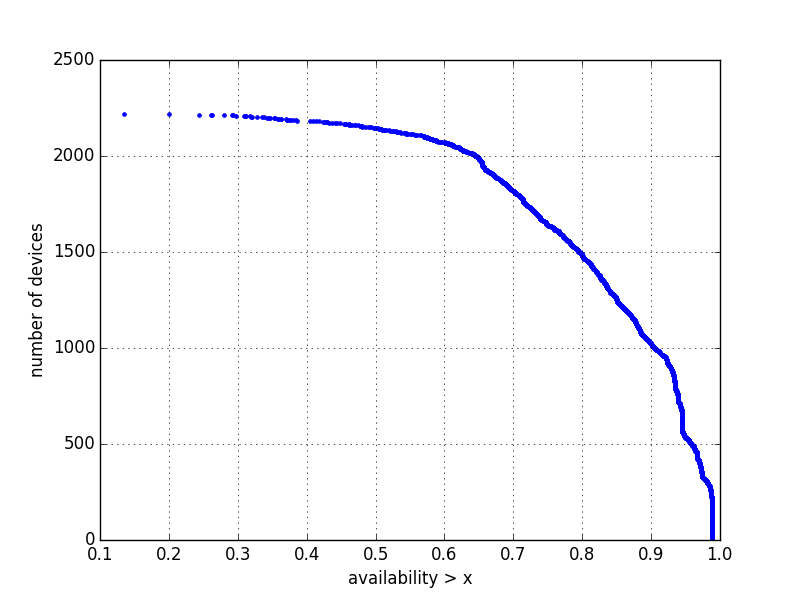
\includegraphics[width=\linewidth]{figures/250-test_dw-availability-CDF.png}
  \caption{Availability by device}
  \label{fig:availability-device}
\end{subfigure}
%
\hspace{-1em}
%
\begin{subfigure}[b]{0.5\linewidth}
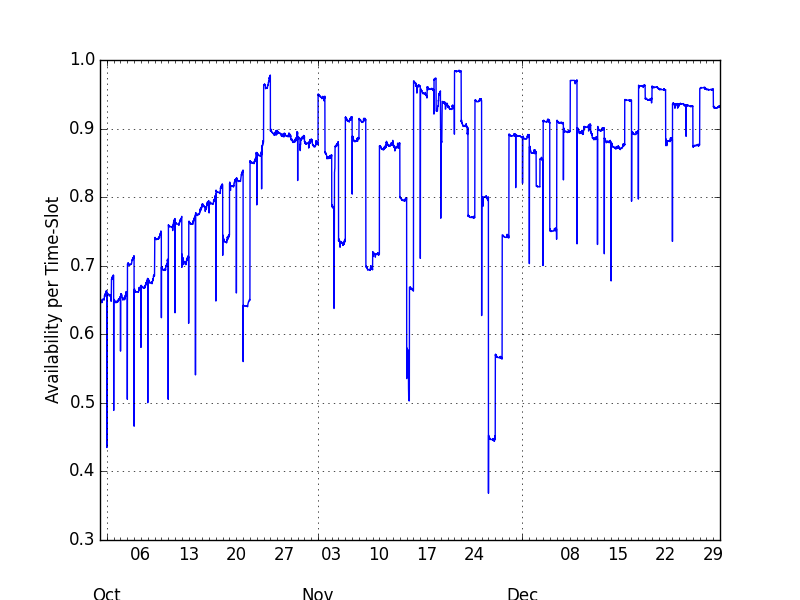
\includegraphics[width=\linewidth]{figures/250-test_dw-availability-by-date.png}
  \caption{Availability by date}
  \label{fig:availability-date}
\end{subfigure}
%\hfill
%
\end{minipage}
\caption{Availability, based on gateway device responsiveness. }
\label{fig:availability}
% created using docs/metadata-separated.log
\end{figure}

% remove weird dates with very low machines
On exploring \control 4, we noticed that the dataset spanned the October-December period, but for the first week there were 15000 unique devices reporting their usage statistics, while after the first week, the number dropped to 5000. Furthermore, \control 5 and \control 6 reported usage for 5000 devices in the month of November, but only a 100 devices in December. We did not want stray devices impacting our measure of availability, therefore we sliced the \control datasets to monthly date ranges with a minimum of 4000, or at least half the total unique devices present.
% why 4000? --- eyeballing availability plots -- 3k to 4k seemed to be the right choice for control4

%final datasets for each control, each month, and full
%\sg{after sanitization, we can either compare test to each control in the same time range and draw agg conclusions, or do it by month, or combo it into a huge control set and compare it with test set}
%\sg{Present results for full sets, unless there is a significant difference in any trends or distributions}
Finally, we sliced the sanitized \test set based on the date range of each individual \control set for comparison. We compared each of these tests individually to ensure that there are no outliers. We refer to the \test and \control sets in this case simply as datasets $1-8$. To analyze data by each month, we also sliced and combined the sanitized data to give us \control and \test data for October, November, and December, referred to as $oct$, $nov$, $dec$. Finally, we combine all \control sets to form a large concatenated dataset over the same date range as the complete \test dataset, and we refer to this simply as $full$. A description of these sanitized sets is provided in table~\ref{tab:sanitized-description} 

\begin{table*}[ht]
\small
\begin{tabular}{|l|l|l|l|l|l|l|l|l|l|l|l|l|}
\hline
\textbf{Dataset}            & set$_1$      & set$_2$      & set$_3$      & set$_4$      & set$_5$      & set$_6$      & set$_7$      & set$_8$      & set$_{oct}$  & set$_{nov}$  & set$_{dec}$  & set$_{full}$ \\ \hline
\textbf{Start Time}         & 2014-09-30  & 2014-10-01  & 2014-10-01  & 2014-11-01  & 2014-11-01  & 2014-11-01  & 2014-11-01  & 2014-12-01  & 2014-10-01  & 2014-11-01  & 2014-12-01  & 2014-09-30  \\ \hline
\textbf{End Time}           & 2014-10-31  & 2014-10-31  & 2014-10-312 & 2014-12-29  & 2014-12-29  & 2014-12-29  & 2014-12-29  & 2014-12-29  & 2014-10-30  & 2014-11-29  & 2014-12-29  & 2014-12-29  \\ \hline
\textbf{Devices$_{\control}$} & 3627                & 4033                & 3969                & 1266                & 3632                & 3852                & 3644                & 4277                & 11629               & 12394               & 13405               & 16015               \\ \hline
\textbf{Devices$_{\test}$}    & 1481                & 1481                & 1481                & 1481                & 1481                & 1481                & 1481                & 1481                & 1481                & 1481                & 1481                & 1481                \\ \hline
\end{tabular}
\caption{Sanitized Dataset Description: Most of our analysis will be based on set$_{full}$ unless otherwise stated }
\label{tab:sanitized-description}
\end{table*}



\todo{Figure~\ref{fig:availability} Make common \textbf{EPS} plot of availability -- 8 control sets (half filtered) + test sets vs availability.}

\sg{Figure~\ref{fig:availability-device} should show why we chose 0.5 as threshold, Figure~\ref{fig:availability-date} should show why we expected 3k-4k sanitized devices per set} 

\todo{Table~\ref{tab:sanitized-description} recheck all numbers and rewrite para accordingly, it seems control4 did not end at just one month - continued till December}

\todo{Table~\ref{tab:sanitized-description} turn it around}